\chapter{構造最適化}\label{ux69cbux9020ux6700ux9069ux5316}

    \section{背景}\label{ux80ccux666f}

構造最適化が何故必要となるかを初めに詳しく記しておく.

    \subsection{VASPの構造最適化ルーチン}\label{vaspux306eux69cbux9020ux6700ux9069ux5316ux30ebux30fcux30c1ux30f3}

図はAlの3315で作成したモデルのtop
viewである.これを緩和させて最安定エネルギーを求める.
このためには内部の原子配置と,外部のセル形状の両方を緩和させる必要がある.
今後これらをそれぞれ内部緩和,外部緩和と呼んでいく.

\begin{center}
\includegraphics[width=150mm]{../.././figs/POSCAR_0_3315_46_Al.png}
\end{center}
一般的な第一原理計算では構造最適化のルーチンが用意されている.

\label{fig:This}
我々が使用しているVASPにおいて用意されているルーチンは表の通りである.

\begin{longtable}[]{@{}llllll@{}}
\toprule
ISIF & force & stress tensor & ions & cell shape & cell
volume\tabularnewline
\midrule
\endhead
0 & yes & no & yes & no & no\tabularnewline
1 & yes & trace only* & yes & no & no\tabularnewline
2 & yes & yes & yes & no & no\tabularnewline
3 & yes & yes & yes & yes & yes\tabularnewline
4 & yes & yes & yes & yes & no\tabularnewline
5 & yes & yes & no & yes & no\tabularnewline
6 & yes & yes & no & yes & yes\tabularnewline
7 & yes & yes & no & no & yes\tabularnewline
\bottomrule
\end{longtable}

\begin{itemize}
\tightlist
\item
  Trace only means that only the total pressure, i.e. the line
  http://cms.mpi.univie.ac.at/vasp/guide/node112.html
\end{itemize}

VASPの呼称ではionが内部原子を,cellが外部セル形状を意味する.

例えば,ISIF=0ではion=yes,cell shape,
volume=noとなっており,内部緩和は行うが,cellの形状と体積はfixしたままである.

ISIF=7では,内部緩和をおこないセルは形状を保ったまま,体積を変化させる.
ところが,セル形状を保ったままでの体積変化は,等方的に緩和させるようである.

図はISIF=3で計算した場合の結果を示した.
\begin{center}
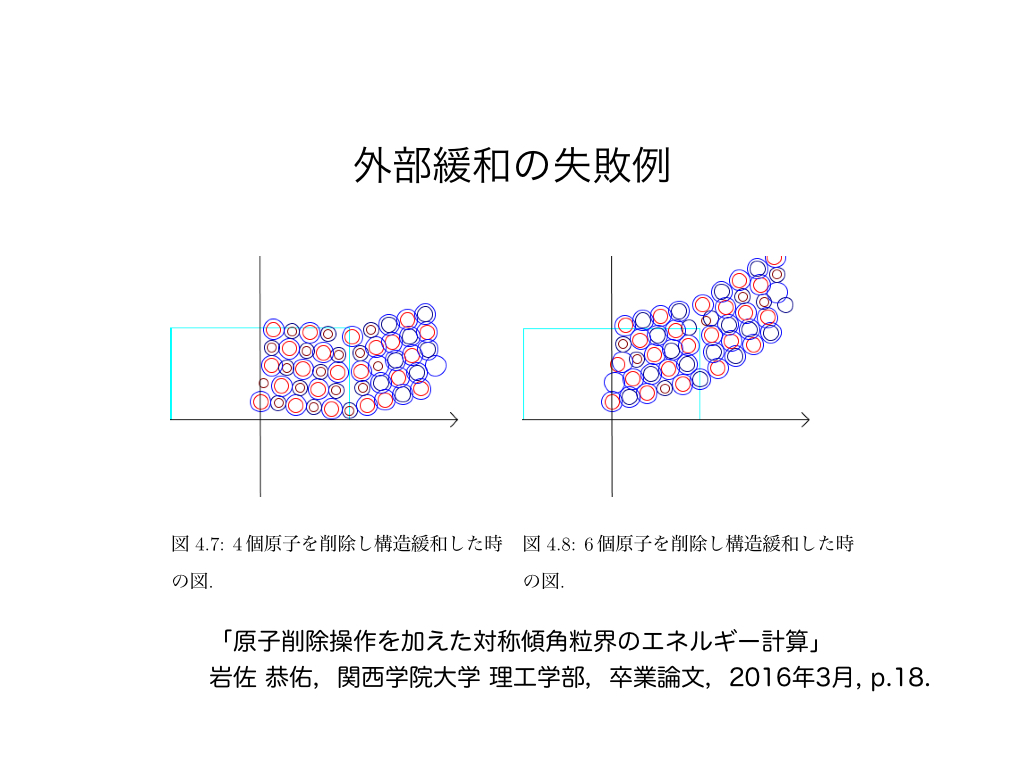
\includegraphics[width=150mm]{../.././figs/thesis/thesis_004.jpeg}
\end{center}


\label{fig:}
粒界構造のモデルで用いられる,いびつな立方晶のセル形状から
外部,内部緩和を全て自動で緩和させると, 外部セル形状が極端に変形する.
いびつな立方晶のセル形状を保ったまま
それぞれの長さを変えるようなスイッチは用意されていない.
したがってこれを行うルーチンは,独自に開発する必要がある.

    \subsection{POSCARのファイル構造}\label{poscarux306eux30d5ux30a1ux30a4ux30ebux69cbux9020}

モデルとしてCu\_3315をつかう.
これは系のサイズが小さく,第一原理計算VASPの計算時間が
少なく済むからである.

いかに,VASPの計算に投入する原子の情報を集めた
POSCARと呼ばれるファイルである.

\begin{verbatim}
> head POSCAR_0_3315_46_Al
(Al) Source:.POSCAR_0;Expand:3,3,1;Shaped;Rotate:1/5,22.62[degrees];Mirrorred;Shaped2;Cut:0.81715-0.84984
   1.00000000000000
  19.8145937137    0.0000000000    0.0000000000
   0.0000000000   10.3035887311    0.0000000000
   0.0000000000    0.0000000000    4.0414000000
46
Selective dynamics
Direct
   0.6000000000    0.0384615385    0.5000000000 T T T
   0.5800000000    0.2307692308    0.0000000000 T T T
...以下略
\end{verbatim}

3行目から5行目にかかれた3次元ベクトルがcellの外形のa,b,cを 示している.
\(a\)が図では\(x\)軸,\(b\)が\(y\)軸,\(c\)が\(z\)軸のベクトルの
カーテシアン座標をオングストロームで示している.

さらに次の行にそのセルに含まれる原子の数(=46)が表記されている.
それ以降の2行にキーワードがあり,
それ以下には,それぞれの原子のローカルな相対座標が記されている.
これがPOSCARファイルの構造である.

    \subsection{vasp計算の結果}\label{vaspux8a08ux7b97ux306eux7d50ux679c}

    図はAl\_3315のセルサイズ変化によるエネルギー表面を示している.

\begin{figure}[H][htbp]
\centering
\begin{center}
\includegraphics[width=150mm]{../.././figs/Al_3315_surface.png}
\end{center}
\caption{}

\label{fig:}
\end{figure}

    このエネルギー表面の特徴は次の通りである. 1. x=-8..0 1. y=-2..2 1.
x軸方向の変化は大きい. 1. y軸方向の変化はねじれている.すなわち 1.
x=0ではyの増加につれて上がっていくが, 1.
x=-8ではyの増加につれて下がっている 1.
x=-4の直線上でminimumを取っている.

もう少し細かくエネルギー計算をした場合と,もう少し荒くエネルギー計算をした場合で,
最小値やその位置が大きく変わるかどうかを検証する必要がある.

また,この例では最小値の囲い込みがうまくいっているが,初期には
囲い込まれていなかった.したがって,どの程度の余裕をもって
計算の初期値とするかを決定する必要がある.

    これは,計算によって得られた値を3次元プロットした結果である.

\begin{longtable}[]{@{}rrr@{}}
\toprule
x & y & E\tabularnewline
\midrule
\endhead
-8 & -2 & 0.70408\tabularnewline
-8 & 0 & 0.62402\tabularnewline
-8 & 2 & 0.58637\tabularnewline
-4 & -2 & 0.54846\tabularnewline
-4 & 0 & 0.52160\tabularnewline
-4 & 2 & 0.52985\tabularnewline
0 & -2 & 0.58105\tabularnewline
0 & 0 & 0.59046\tabularnewline
0 & 2 & 0.63185\tabularnewline
\bottomrule
\end{longtable}

これらの値は,粒界モデルのx軸,y軸を変化させ,セル形状を固定した状態で,内部緩和をおこないエネルギー計算を行っている.
これをfittingして,最安定構造を求めるには次のMapleスクリプトで得られる.

\begin{verbatim}
x0:=-4;y0:=0;
with(stats): data:=[xx,yy,zz]: 
fit1:=fit[leastsquare[[x,y,z], 
    z=a1+a2*(x-x0)+a3*(y-y0)+a4*(x-x0)*(y-y0)+
      a5*(x-x0)^2+a6*(y-y0)^2, 
    {a1,a2,a3,a4,a5,a6}]](data);

fit1 := z = .5026144708-0.4629870219e-2*x-0.7128049500e-2*y+
(0.5266188957e-2*(x+4))*y+0.5395943477e-2*(x+4)^2+0.4563284219e-2*y^2
\end{verbatim}

これで求められた関数fit1をx,yで微分し,連立方程式として解くと

\begin{verbatim}
e1:=diff(f1(x,y),x);
e2:=diff(f1(x,y),y);
s1:=solve({e1,e2},{x,y});
       0.03853767760 + 0.005266188957 y + 0.01079188695 x
      0.01393670633 + 0.005266188957 x + 0.009126568438 y
              {x = -3.933335758, y = 0.7425554356}
subs(s1,f1(x,y));
                          0.5183331423
\end{verbatim}

として求めることが可能である.

この最安定構造をできるだけ少ない手数で求めることが開発目標となる.

ところがこれらの結果はVASPによって得られたエネルギー値を示している.
VASPはこの程度の計算であっても,一点の計算に現有の設備でAlで1時間50分程度,Cuの計算では6時間程度が必要となる{[}参照:藤村{]}.
これを開発段階で使っていては応答時間が長すぎるため,現実的ではない.
そこで,計算時間が劇的に短い経験ポテンシャルであるEAMを使って開発を進める.

    \section{手法}\label{ux624bux6cd5}

\subsection{EAM}\label{eam}

eamはembedding atom methodと呼ばれる原子間のポテンシャルで...
ここ書きや.

    \subsection{ディレクトリー構造}\label{ux30c7ux30a3ux30ecux30afux30c8ux30eaux30fcux69cbux9020}

pseudo\_vaspに関連するファイルを作成する.

\begin{verbatim}
tree pseudo_vasp
.
├── CODE_OF_CONDUCT.md
├── Gemfile
├── Gemfile.lock
├── LICENSE.txt
├── README.md
├── Rakefile
├── bin
│   ├── console
│   └── setup
├── docs
├── exe
│   └── pseudo_vasp
├── lib
│   ├── pseudo_vasp
│   │   ├── eam.rb
│   │   └── version.rb
│   └── pseudo_vasp.rb
├── pseudo_vasp.gemspec
└── test
    ├── POSCAR_0
    ├── POSCAR_0_3315_46_Al
    ├── cell_bracket.rb
    ├── cell_relaxation.rb
    ├── eam.rb
    ├── pseudo_vasp_test.rb
    └── test_helper.rb

6 directories, 21 files
\end{verbatim}

これは,ruby gemsのライブラリーの標準構成で,

\begin{quote}
bundler gem init -b pseudo\_vasp
\end{quote}
で作成された.

libの中にeamポテンシャルのcodeが入っている.
testにはそれぞれの計算駆動codeを置いている. それらは,

\begin{verbatim}
eam.rb                eamのe-v曲線
cell_relaxation.rb    外部cell変形のエネルギー
cell_bracket.rb       cell緩和の囲い込み
\end{verbatim}

である.

    \section{結果}\label{ux7d50ux679c}

    \subsection{囲い込み}\label{ux56f2ux3044ux8fbcux307f}

一般的な数値計算における最適化の最初の一歩は解の囲い込みである.
数値計算のバイブルNumerical
recipeにはそのための標準ルーチンとしてmnbrakが用意されている.
そこで,まずはこれをrubyで実装した.

"Numerical Recipes in C", by W.H.Press他,(技術評論社, 1993), pp.285-289

結果は次の通りである.

\begin{verbatim}
[1]init range:   1.00000-   1.02000
 init_x:=[ 1.0200,  1.0000,  0.9676]; init_y:=[ 0.2414,  0.0000,  1.1178];
final_x:=[ 1.0200,  1.0000,  0.9676];final_y:=[ 0.2414,  0.0000,  1.1178];
n_calc:   3

[2]init range:   0.98000-   0.99000
 init_x:=[ 0.9800,  0.9900,  1.0062]; init_y:=[ 0.3041,  0.0454,  0.0404];
final_x:=[ 0.9900,  0.9982,  1.0062];final_y:=[ 0.0454, -0.0033,  0.0404];
n_calc:   4

[3]init range:   0.97000-   0.97500
 init_x:=[ 0.9700,  0.9750,  0.9831]; init_y:=[ 0.9058,  0.5516,  0.1947];
final_x:=[ 0.9898,  0.9974,  1.0008];final_y:=[ 0.0475, -0.0034,  0.0027];
n_calc:   6

[4]init range:   0.97000-   0.97200
 init_x:=[ 0.9700,  0.9720,  0.9752]; init_y:=[ 0.9058,  0.7497,  0.5377];
final_x:=[ 0.9873,  0.9981,  1.0068];final_y:=[ 0.0900, -0.0034,  0.0465];
n_calc:   6

[5]init range:   0.97000-   0.97100
 init_x:=[ 0.9700,  0.9710,  0.9726]; init_y:=[ 0.9058,  0.8252,  0.7055];
final_x:=[ 0.9864,  0.9984,  1.0088];final_y:=[ 0.1075, -0.0032,  0.0688];
n_calc:   6

[6]init range:   0.97000-   1.00100
 init_x:=[ 0.9700,  1.0010,  1.0512]; init_y:=[ 0.9058,  0.0036,  0.8926];
final_x:=[ 0.9700,  1.0010,  1.0512];final_y:=[ 0.9058,  0.0036,  0.8926];
n_calc:   3
\end{verbatim}

テストケース{[}1{]},{[}6{]}は,計算結果からわかる通り初期値とさらにcx =
bx + GOLD*(bx-ax)で求められる値を計算するだけで囲い込みが成功している.

テストケース{[}2{]}は,初期の3点では囲い込んでいるかがわからず中簡点を追加計算することで求めている.
この様子を図に示した.初期の3点は赤丸で,最終結果の3点を青丸で示している.初期の3点の中間に,青丸で示した4つ目の計算結果が追加されている.

一方,テストケース{[}4{]}-{[}6{]}は囲い込みが初期の3点ではうまくいっておらず,だいぶ外側に外れた位置での計算が必要となっている.初期値のステップの大小によるロスはmnbrakの計算ルーチンによってうまく回避されている(図(b),(c)).
\begin{center}
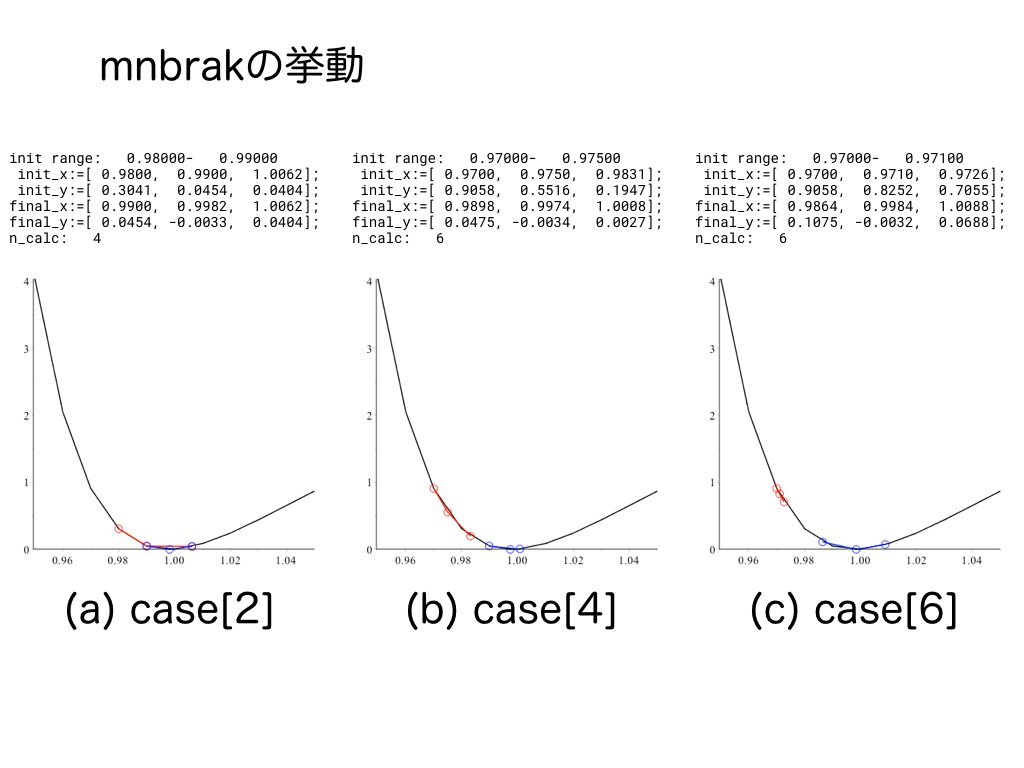
\includegraphics[width=150mm]{../.././figs/thesis_006.jpeg}
\end{center}
初期値の取り方を間違うと最大6になるが,

\label{fig:}
概ね,囲い込みは効率良くmnbrakによって可能であることが確認できた.
そこで,このルーチンをそのまま使ってこの後の開発を進めることとした.

    \subsection{界面エネルギーへの変換}\label{ux754cux9762ux30a8ux30cdux30ebux30aeux30fcux3078ux306eux5909ux63db}

次に示すコードは計算サーバに用意されているRakefile内で
VASP計算結果から表面エネルギーを求めるメソッドである.

\begin{verbatim}
def calc_df_es(n_atom, lat_c)
  _status, stdout, = systemu("tail inner_*.o* |grep 'F='")
  df = stdout.scan(/F=(.+) E0/)[0][0].to_f
  de = df - n_atom * -3.739501247
  ss = lat_c[1] * lat_c[2]
  es = de / ss * 1.60218 * 10 / 2
  df.to_s + ' ' + es.to_s + "\n"
end
\end{verbatim}

ここで,lat\_c{[}1{]},
lat\_c{[}2{]}に\(a,b\)軸の値が,ssに界面の面積が,
dfにVASPで求められたエネルギー値が,
n\_atomに原子数が入っている.esでは得られた界面エネルギー(\(dE/S\))を
"{[}eV/A\^{}2{]}"から"{[}J/m\^{}2{]}"に変換している.
分母の2はユニットセル内に2枚の界面があるためにその数で割っている.

この出力をとると,

\begin{verbatim}
#i  j  dE  
  -6   -1   18.62572   10.20055    4.04140 -168.48987 0.6854160866046254
  -6    0   18.62572   10.30359    4.04140 -168.56613 0.6638909918907453
  -6    1   18.62572   10.40662    4.04140 -168.59626 0.6515787808351412
...
\end{verbatim}

となる.これに対応して,pseudo\_vaspの出力を調整して,

\begin{verbatim}
  -2   -2  19.81459   10.30359    4.04140 -150.03001   0.24146     
  -2   -1  19.81459   10.30359    4.04140 -150.15656   0.23390     
  -2    0  19.81459   10.30359    4.04140 -150.15225   0.23173     
  -2    1  19.81459   10.30359    4.04140 -150.04017   0.23388     
  -2    2  19.81459   10.30359    4.04140 -149.84182   0.23938     
  -1   -2  19.81459   10.30359    4.04140 -150.32396   0.22713     
  -1   -1  19.81459   10.30359    4.04140 -150.43100   0.22055     
  -1    0  19.81459   10.30359    4.04140 -150.41091   0.21914     
  -1    1  19.81459   10.30359    4.04140 -150.28600   0.22187     
  -1    2  19.81459   10.30359    4.04140 -150.07716   0.22781     
   0   -2  19.81459   10.30359    4.04140 -150.39718   0.22193     
   0   -1  19.81459   10.30359    4.04140 -150.48888   0.21605     
   0    0  19.81459   10.30359    4.04140 -150.45633   0.21517     
   0    1  19.81459   10.30359    4.04140 -150.32128   0.21828     
   0    2  19.81459   10.30359    4.04140 -150.10416   0.22450     
   1   -2  19.81459   10.30359    4.04140 -150.33460   0.22221     
   1   -1  19.81459   10.30359    4.04140 -150.41477   0.21682     
   1    0  19.81459   10.30359    4.04140 -150.37283   0.21628     
   1    1  19.81459   10.30359    4.04140 -150.23011   0.21963     
   1    2  19.81459   10.30359    4.04140 -150.00670   0.22599     
   2   -2  19.81459   10.30359    4.04140 -150.19187   0.22564     
   2   -1  19.81459   10.30359    4.04140 -150.26371   0.22057     
   2    0  19.81459   10.30359    4.04140 -150.21493   0.22024     
   2    1  19.81459   10.30359    4.04140 -150.06662   0.22370     
   2    2  19.81459   10.30359    4.04140 -149.83865   0.23011
\end{verbatim}

とした.このエネルギー表面を描画すると次のとおりとなる.

\begin{figure}[H][htbp]
\centering
\begin{center}
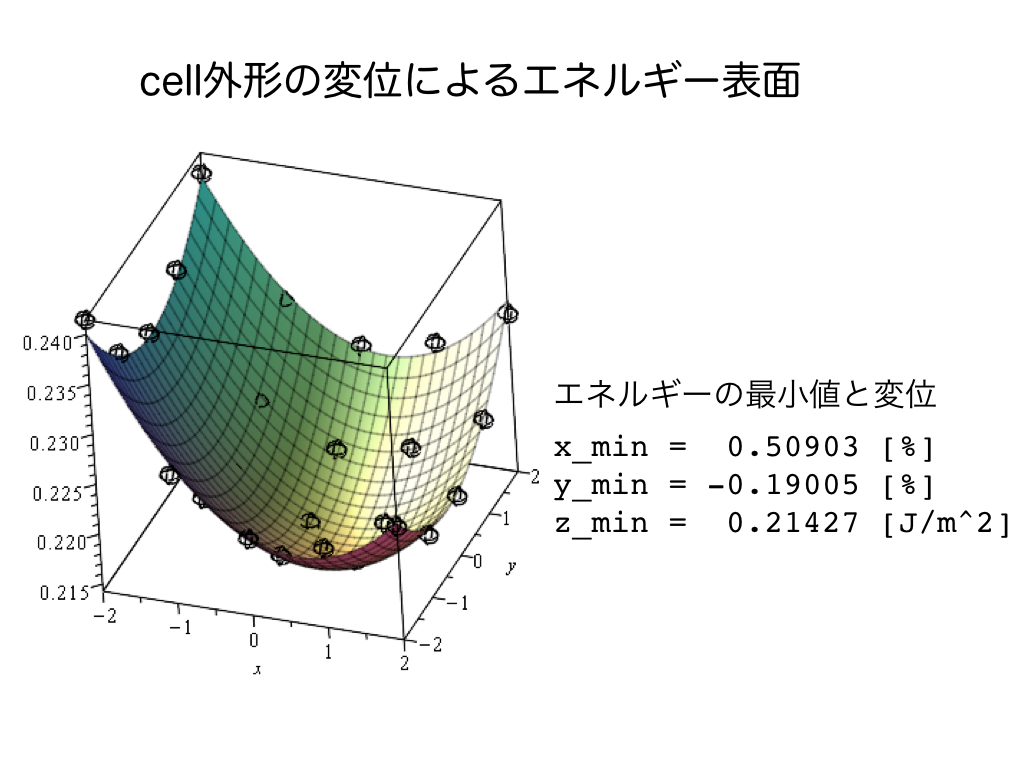
\includegraphics[width=150mm]{../.././figs/thesis/thesis_007.jpeg}
\end{center}
\caption{cell外形の変位によるエネルギー表面.\label{spandata-label}}

\label{fig:}
\end{figure}

    cellの外形変位によるエネルギー表面は上図のようになる.ここで,VASPの結果との違いは次のとおりである.
1.
VASPではx=-8..0で囲い込まれているのに対して,EAMではx=-2..2で囲い込まれている
1.
EAMの結果はx=2およびx=-2において,yの変化に対してどちらも2次の項が優勢である.
1.
VASPの結果は,yの変化に対して1次の項も大きく寄与しており,さらにその傾きが逆向きに効いている.

これが後ほど聞いてくるかもしれないので留意しておく.

    \section{2次元での最小化}\label{ux6b21ux5143ux3067ux306eux6700ux5c0fux5316}

\subsection{最小計算数での試行}\label{ux6700ux5c0fux8a08ux7b97ux6570ux3067ux306eux8a66ux884c}

次に2次元の最小化をすることになる.
一般的なテキストでは,この後,多次元の最小化を行う,共役勾配法などが使われるが,
我々の問題では2次元と,非常に少ない次元数であるので,このままmnbrakを使って,
x,yで最小化を試みる.

mnbrakの最初の実装では,

\begin{verbatim}
def func(ax)
  $n_calc+=1
  $model.set_cell_size(ax)
  $model.total_energy+150.45633275921924
end

# mnbrak, coding from Num Recipe in C
def mnbrak(ax, bx)
  printf("init range:%10.5f-%10.5f\n",ax,bx)
  $n_calc = 0

  fa = func(ax)
\end{verbatim}

としていた.これをy軸方向への変位を扱えるように,次の様に変更した.

\begin{verbatim}
def func_x(ax,ay=1.0)
  $n_calc+=1
  $model.set_cell_size(ax,ay)
  $model.total_energy+150.45633275921924
end

def func_y(ay, ax=1.0) # note the order of ax, ay 
  $n_calc+=1
  $model.set_cell_size(ax,ay)
  $model.total_energy+150.45633275921924
end

# mnbrak, coding from Num Recipe in C
def mnbrak(ax, bx, method_func=method(:func_x))
  printf("init range:%10.5f-%10.5f\n",ax,bx)
  $n_calc = 0

  fa = method_func.call(ax)
\end{verbatim}

具体的な変更箇所は, 1. 呼び出す関数を引数として受け取り, 1.
それを明示的に呼び出す(call)

である.これによって,x軸とy軸に沿った囲い込みを行えるように変更している.
これによって,mnbrakのcodeを書き換えること無く, 関数func\_x,
func\_yに変位の操作を委ねている.
これに従ってmnbrakを2次元で行うように変更すると, 呼び出し方は,

\begin{verbatim}
  x_min =  mnbrak(1.0, 1.02, method(:func_x) )
  y_min =  mnbrak(1.0, 1.02, method(:func_y) )
\end{verbatim}

と変更することで

\begin{verbatim}
math := <<   2.00000|   0.00000|   0.24140>,
<   0.00000|   0.00000|   0.00000>,
<  -3.23607|   0.00000|   1.11778>,
<   0.00000|   2.00000|   0.35218>,
<   0.00000|   0.00000|   0.00000>,
<   0.00000|  -3.23607|   0.37768>>;
\end{verbatim}

と数値が得られる.

これからfittingを行うと

\begin{figure}[H][htbp]
\centering
\begin{center}

\includegraphics[width=150mm]{../.././figs/thesis/thesis_008.jpeg}
\end{center}
\caption{x,y軸方向のmnbrakによる最安定化の試行.¥label\{spandata-label\}}

\label{fig:}
\end{figure}

となる.これはcalc\_e\_surfでの結果と違っている.
なぜなら,エネルギー表面は最安定ではなく, 鞍点となっているからである.
したがって,もうすこし,工夫が必要である.

    \subsection{手動による計算点の追加}\label{ux624bux52d5ux306bux3088ux308bux8a08ux7b97ux70b9ux306eux8ffdux52a0}

先ほどのグラフをみると,鞍点になった原因は,
範囲の最小値ペアと最大値ペアのところで,
値が小さいと判断されていたためと考えられる.

そこで,まずは

\begin{verbatim}
  print "indicate additional calc point [x,y]:"
  line = gets
  x,y=line.chomp.split(',')
  $model.set_cell_size(x.to_f/100.0+1.0,y.to_f/100.0+1.0)
  z = $model.total_energy+150.45633275921924
\end{verbatim}

として,この値を手動で追加して どのようになるかを確かめた.

\begin{figure}[H][htbp]
\centering
\begin{center}
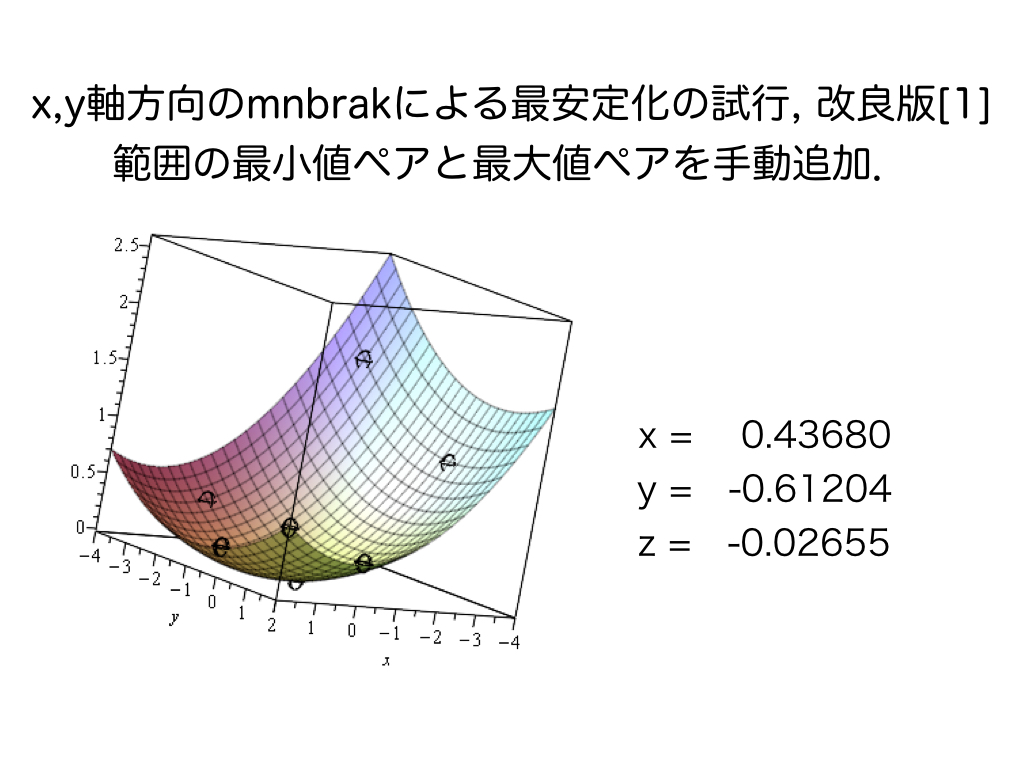
\includegraphics[width=150mm]{../.././figs/thesis/thesis_009.jpeg}
\end{center}
\caption{範囲の最小値ペアと最大値ペアの手動追加.\label{spandata-label}}

\label{fig:}
\end{figure}

その結果は,安定的なエネルギー表面が描画できている.
さらに,fittingして求めた関数での最小値は,
微小変位で埋め尽くして計算した値と,最安定の
値は違っているが,最安定の場所はそれほど悪くない.

また,エネルギー計算の回数は5+2で7である.
これは,一般的な2次元で網羅的に計算する3x3の9点よりも 少ない.

    \subsection{自動での追加}\label{ux81eaux52d5ux3067ux306eux8ffdux52a0}

先ほどの手動による計算点の追加では,手間がかかる.
そこで,計算点は増えるが,自動で計算点を追加するようにcodeを 改良した

\begin{figure}[H][htbp]
\centering
\begin{center}
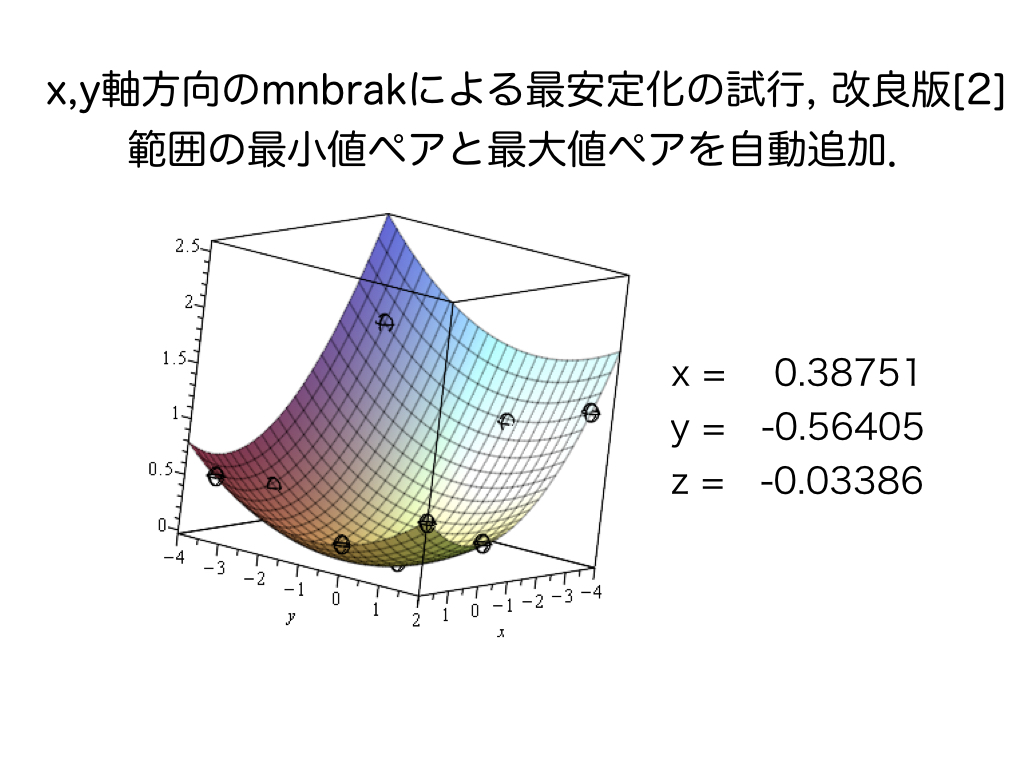
\includegraphics[width=150mm]{../.././figs/thesis/thesis_010.jpeg}
\end{center}
\caption{範囲の最小値ペアと最大値ペアを自動追加.¥label\{spandata-label\}}

\label{fig:}
\end{figure}

この結果は,手動で追加した結果を再現している.しかし,
エネルギー計算の回数を減らしているのでは無いので,
やはり工夫が必要であろう.

    \section{問題の見直し}\label{ux554fux984cux306eux898bux76f4ux3057}

問題は,囲い込みがうまく行っていれば,9回程度で
計算が終了するが,そうでなければ余計な計算がかかることである.

そこで,問題をもういちど見直すことにした.
要は,外部緩和の計算をできるだけ減らしたいということである.
もう一度,Alの計算結果を精査してみた.

\begin{longtable}[]{@{}lrr@{}}
\toprule
/Users/bob/Github/boundary/bob/data/whole\_data/ & x & y\tabularnewline
\midrule
\endhead
0\_5s/vasp\_res\_0\_3315\_46 & -4 & 1\tabularnewline
0\_5s/vasp\_res\_0\_6615\_108 & -8 & 1\tabularnewline
0\_5s/vasp\_res\_0\_6615\_148 & -6 & 1\tabularnewline
0\_5s/vasp\_res\_0\_6615\_188 & -4 & 0\tabularnewline
0\_7s/vasp\_res\_0\_4417\_88 & -8 & 0\tabularnewline
0\_7s/vasp\_res\_0\_8817\_130 & -6 & 0\tabularnewline
0\_7s/vasp\_res\_0\_8817\_186 & -4 & 0\tabularnewline
0\_7s/vasp\_res\_0\_16417\_386 & -2 & 0\tabularnewline
0\_9s/vasp\_res\_0\_5519\_148 & -8 & 1\tabularnewline
0\_9s/vasp\_res\_0\_5519\_152 & -4 & 0\tabularnewline
0\_9s/vasp\_res\_0\_101019\_310 & -4 & 0\tabularnewline
\bottomrule
\end{longtable}

energyがminiに鳴っている,x,yのペアの一覧表をつくってください.

    \section{自動原子削除の実装}\label{ux81eaux52d5ux539fux5b50ux524aux9664ux306eux5b9fux88c5}

粒界生成において,回転,並びに鏡映操作を行った後の原子配置を図に示した.

\begin{center}
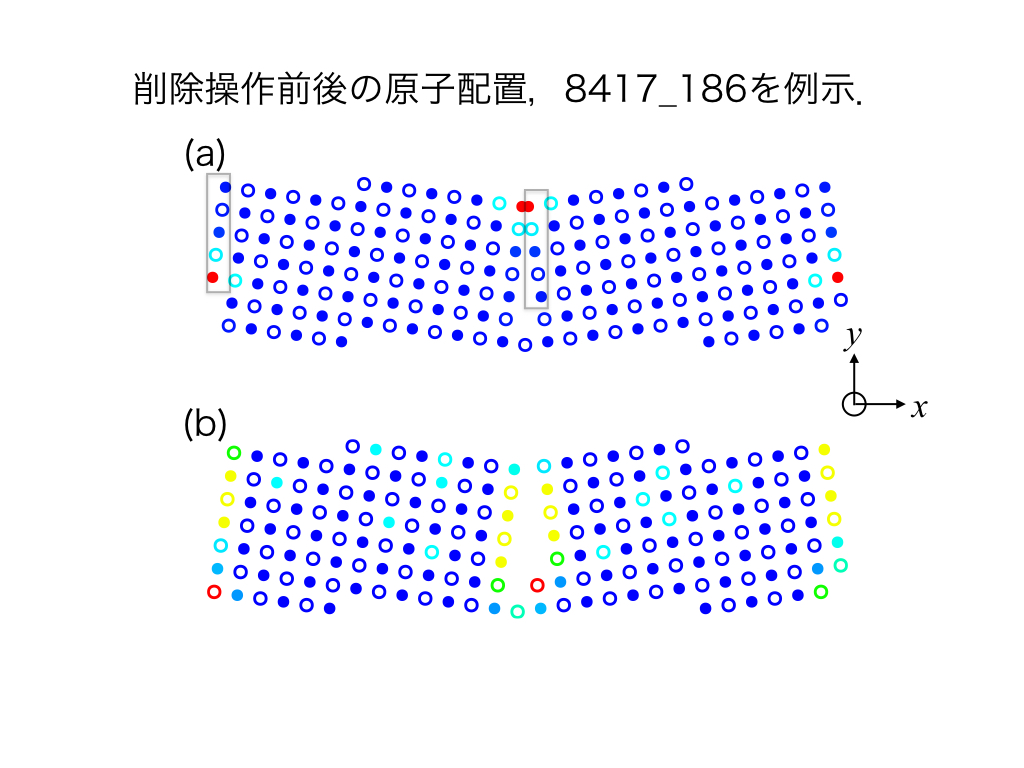
\includegraphics[width=150mm]{../.././auto_delete/auto_delete_002.jpeg}
\end{center}
削除操作前後の原子配置,8417\_186を例示.

\label{fig:}

ここでは,8417\_186を例にしている.8417の数字は粒界系全体の構造を表している.それぞれ,x=8,
y=4, z=1およびtan
\(\theta=1/7\)を意味しており,x軸方向に8x2層,y軸方向に4x2層の層を保持している.

削除操作は,このx=0, およびx=0.5つまり,系の端と真ん中あたりにある
粒界近傍において,原子が詰まりすぎているのを解消するために行う操作である.
枠線で囲った領域の原子を削除する.
これまではVestaという表示ソフトを使って,原子サイトナンバーを手動で確認し,
モデル作成司令ファイル(modeler\_8417など)に記述する必要があった.
これを自動化しようというのがここで目指す開発コードである.

    \section{energyおよびnlによる抽出}\label{energyux304aux3088ux3073nlux306bux3088ux308bux62bdux51fa}

    当初,eamのプログラムコードを流用して原子のエネルギー(:ene, energyの略)
あるいは配位数(:nl,neighbour listを意味)を使った選別を試みた.
近傍の原子を取り出すと,

\begin{verbatim}
   4   28.86278    8.28733    2.02070  11   -2.65182  0.738    3.08007   -5.73189 0.54
   5   28.57701   10.28772    0.00000  13    0.23319  3.623    7.50972   -7.27653 1.03
   6   28.29124   12.28812    2.02070  14   12.27927 15.669   21.86782   -9.58855 2.28
   8   55.72518    6.00117    2.02070  14   12.27927 15.669   21.86782   -9.58855 2.28
  94   55.43941    8.00156    0.00000  13    0.23319  3.623    7.50972   -7.27653 1.03
  95   55.15364   10.00195    2.02070  11   -2.65182  0.738    3.08007   -5.73189 0.54
 103   27.14816    8.28733    2.02070  11   -2.65182  0.738    3.08007   -5.73189 0.54
 104   27.43393   10.28772    0.00000  13    0.23319  3.623    7.50972   -7.27653 1.03
 105   27.71970   12.28812    2.02070  14   12.27927 15.669   21.86782   -9.58855 2.28
 106    0.28577    6.00117    2.02070  14   12.27927 15.669   21.86782   -9.58855 2.28
 192    0.57154    8.00156    0.00000  13    0.23319  3.623    7.50972   -7.27653 1.03
 193    0.85731   10.00195    2.02070  11   -2.65182  0.738    3.08007   -5.73189 0.54
\end{verbatim}

が選択される.これは,6列目に記されたeneryを基準に選別したものである.
しかし,サイト番号7に対応する

\begin{verbatim}
   7   56.01095    4.00078    0.00000  12   -3.39000 -0.000    1.79000   -5.18000 0.35
\end{verbatim}

がこれらの選別基準では最安定原子と同じ環境であるため,選択から外れてしまう.

    \section{x位置による選別}\label{xux4f4dux7f6eux306bux3088ux308bux9078ux5225}

そこで,x座標による選別を実装した.
初期のcodeがわかりやすいので,そのまま記すと次のようになる.

\begin{verbatim}
a_length =   56.0109463716
dx = a_length/(32+2)
a_half = a_length/2.0
if x_pos < dx or  (x_pos > a_half and x_pos < a_half + dx)
    printf("%10.5f: ", x_pos/a_length)
\end{verbatim}

削除領域の幅(dx)は層数から計算する.
中心の長さはx軸の長さ(a\_length)から計算している. これらの領域
\textgreater{} 0 \textless{} x\_pos \textless{} dx

\begin{quote}
a\_half \textless{} x\_pos \textless{} a\_half + dx
\end{quote}
を選別するのがif文以下のところである.

こうして得られた削除原子のx\_posを取り出すと,

\begin{verbatim}
> ruby auto_delete.rb converted_poscar.txt 
divide num:   32
a length  :   56.0109463716
normal dx :    0.03125
       dx :    1.75034
   2:    0.53061   29.72009
   3:    0.52551   29.43432
   4:    0.52041   29.14855
   5:    0.51531   28.86278
   6:    0.51020   28.57701
   7:    0.50510   28.29124
 107:    0.00510    0.28577
 192:    0.03061    1.71462
 193:    0.01020    0.57154
 194:    0.01531    0.85731
 195:    0.02041    1.14308
 196:    0.02551    1.42885
\end{verbatim}

となる.ここでは,2番,192番は消したくない原子である.
これは,モデルのサイズによって変わる. この調整をdivide
numによって自動計算からするか,
あるいは10原子削除というように外部入力として入れるかを検討する必要がある.

    \section{POSCARファイルの仕様}\label{poscarux30d5ux30a1ux30a4ux30ebux306eux4ed5ux69d8}

粒界の原子座標の入出力は第一原理計算ソフトVASPのPOSCARファイルを通じて行う.
そこで,POSCARファイルを直接あつかうPOSCAR classを設計する.

今後code内での変数名を用語を一致させるため,VASP標準の単語を使用する.
POSCARの仕様は \textgreater{}
http://cms.mpi.univie.ac.at/vasp/guide/node59.html

あるいはVASP manual, pp.43-4に解説されている.

\begin{verbatim}
Cubic BN         # comment line ('name' of the system)
   3.57          # universal scaling factor ('lattice constant')
 0.0 0.5 0.5     # lattice vectors
 0.5 0.0 0.5  
 0.5 0.5 0.0
   1 1           # number of atoms per atomic species (one number for each atomic species)
Selective dynamics  # 7th
Cartesian           # 7th or 8th
 0.00 0.00 0.00 T T F
 0.25 0.25 0.25 F F F
Cartesian
 0.01 0.01 0.01
 0.00 0.00 0.00
optionally predictor-corrector coordinates 
   given on file CONTCAR of MD-run
  ....
  ....
or
Cubic BN
   3.57
 0.0 0.5 0.5
 0.5 0.0 0.5
 0.5 0.5 0.0
   1 1
Direct
 0.00 0.00 0.00 
 0.25 0.25 0.25
\end{verbatim}

1から6行目に書かれた内容は上記の例にコメントで記した.

7行目は省かれる場合がある.これがあると原子ごとに設定ができる.

The seventh line switches to 'Selective dynamics' (only the first
character is relevant and must be 'S' or 's'). This mode allows to
provide extra flags for each atom signaling whether the respective
coordinate(s) of this atom will be allowed to change during the ionic
relaxation. This setting is useful if only certain 'shells' around a
defect or 'layers' near a surface should relax. Mind: The 'Selective
dynamics' input tag is optional: The seventh line supplies the switch
between cartesian and direct lattice if the 'Selective dynamics' tag is
omitted.

と説明されている.

さらに,7 or
8行目では,これ以降の原子座標の記述法としてCartesianあるいはDirectを指定する.
次の行から原子数分の座標が記される.

Directの場合は,原子位置\(\overrightarrow{R}\)は, \[
\overrightarrow{R} = x_1 \overrightarrow{a}_1 +
x_2 \overrightarrow{a}_2 +
x_3 \overrightarrow{a}_3
\]
で指定される.ここで,\(\overrightarrow{a}_{1 \dots 3}\)は三つの基底ベクトルを指す.そして,
\(x_{1 \dots 3}\)が原子座標に記された,小数点数での値である.

Cartesianの場合は, \[
\overrightarrow{R} = s \,
\left(\begin{array}{cc}
x_1\\
x_2\\
x_3
\end{array}\right)
\] で,\(s\)は2行目にかかれているuniversal scaling factorである.
その他の箇所の説明は今回使用しないので,省略する.

これらの記述に基づいて,それぞれの変数名を

\begin{verbatim}
Cubic BN         # comment
   3.57          # scaling_factor
 0.0 0.5 0.5     # lat_vec[0][0..2]
 0.5 0.0 0.5     # lat_vec[1][0..2]
 0.5 0.5 0.0     # lat_vec[2][0..2]
   1 1           # n_atoms[0..1]
Selective dynamics  # dynamics_selector
Cartesian           # direct_cartesian_switch
 0.00 0.00 0.00  # pos[0]
 0.25 0.25 0.25  # pos[1]
\end{verbatim}

とする.

    \section{auto\_delete\_poscar}\label{auto_delete_poscar}

前述のPOSCARの情報を読み込むPoscar classを使って
実装したのが次のコードである.

\begin{verbatim}
require './poscar'

file = ARGV[0] || 'POSCAR_0_8417'
poscar = Poscar.new(file)
div = ARGV[1].to_i || 32+2
printf("divide num: %4d\n", div)
printf("a length  : %15.10f\n", a_length = poscar.lat_vec[0][0])
printf("normal dx : %10.5f\n", dx = 1.0/div)

a_half = 0.5
selected = []
poscar.pos.each_with_index do |pos,i_atom|
  x_pos = pos[0]
  if x_pos < dx or  (x_pos > a_half and x_pos < a_half + dx)
    printf("%4d %10.5f\n",i_atom.to_i+1,x_pos)
    selected << i_atom
  end
end

poscar.delete_atoms(selected)
File.open('POSCAR_tmp','w') do |file|
  file.print poscar.poscar_format
end
\end{verbatim}

削除の幅は,原子層の厚さから推測できるように第2入力として指定している.
delete\_atomsはselectedで選ばれた番号の原子をPOSCARから消去する命令である.
POSCAR\_0\_4417に適用した結果は次の通りである.

\begin{verbatim}
> ruby auto_delete_poscar.rb POSCAR_0_4417 18
divide num:   18
a length  :   28.0054731858
normal dx :    0.05556
   3    0.55102
   4    0.54082
   5    0.53061
   6    0.52041
   8    0.51020
  88    0.01020
  91    0.02041
  92    0.03061
  95    0.04082
  96    0.05102
[95, 94, 91, 90, 87, 7, 5, 4, 3, 2]
10
88
\end{verbatim}

削除原子数を指定することを断念した.これには,原子のx-座標でsortして順々に選択していかねばならない.
そのsortを指定領域で実行するコードの記述が難しそうなので,今回は見送っている.

    